\documentclass[11pt]{article}
\usepackage{fullpage}
\usepackage{times}
\usepackage{paralist}
\usepackage[round]{natbib}
\usepackage{color}
\usepackage{graphicx}
\usepackage{float}


\newcommand{\textnl}{\textsl}

\newcommand{\note}[1]{\textit{\small\color{magenta}{#1}}}

\title{Does Proficiency impact the use of cognates in L2?\\[.5em]A Computational Approach}
\author{Liat Nativ \and Advisors: Prof.\ Shuly Wintner and Dr.\ Anat Prior} 
\date{}

\begin{document}
\maketitle
\thispagestyle{empty}

\section{Introduction}

The language of non-native speakers, even highly advanced ones, is different from that of native speakers. One source of such differences is the influence of the speaker's first language (L1) on his or her second language (L2); this is referred to as \emph{transfer effects}. Such transfer is evident, inter alia, in the lexical choices made by non-native speakers. 
%
Our hypothesis in this work is that transfer effects, as reflected by lexical choice, are correlated with the speaker's L2 proficiency. We will employ corpus-based computational methods to investigate this hypothesis.

While the main expected contribution of this work is theoretical, there is also practical motivation for such investigation. By gaining insights into the differences in the language produced by non-native speakers and their correlation with L2 fluency, we can contribute to creating better personalized, L1-based, natural language processing (NLP) solutions. 
A motivation for such personalization can be found, for example, in the work of \cite{heilman-etal-2007-combining},
who suggest that since the process of language 
acquisition inherently differs for first and second-language learners (e.g., grammatical structures are acquired in a much slower rate by second language learners), 
readability assessment should be approached differently for these two populations. 
For similar reasons, the task of \emph{text simplification}, both lexical and grammatical, must be solved differently for native and non-native speakers, most probably taking into account also the speaker's L1. However, to the best of our knowledge, this task is currently addressed uniformly, independently of the target audience.
Summing up, understanding of non-native speakers' lexical choices, combined with the ability to assess their fluency level accordingly,
is fundamental for creating ``personalized'' NLP applications, based on the users' L1 background.

\section{Research Goal}

\emph{Cognates} are words in different languages that have  similar forms and similar meanings due to a common ancestor in some protolanguage. Psycholinguistic research has shown that non-native speakers tend to overuse words that have cognates in their L1.  This tendency has also been established recently on a large scale in a corpus-based computational work \citep{TACL1403}.
Our main goal in the current work is  to show a correlation between a non-native author's choice of cognates and his or her proficiency level in L2 (here, always English). 
We hypothesize that higher proficiency authors will tend to be less influenced by their L1, and therefore use cognates in a manner more similar to that of native speakers.

Usually, this type of study is conducted with a small group of human participants, on which detailed information is collected.  Such psycholinguistic studies are usually focused on a small set of words, and participants are requested to make lexical choices in response to ready-made questioning \citep{prior:2006a,BIL:8852637}.
We aim to investigate how lexical choices reflected by the use of cognates are correlated to L2 fluency on a much larger scale, investigating dozens of cognates that occur in the spontaneous language of hundreds of non-native authors with a variety of L1s.

\section{Previous Work}

Most people in the world are able to express themselves in more than one language \citep{grosjean2012psycholinguistics}, thereby maintaining two or more language systems simultaneously---a task that requires considerable cognitive resources  \citep{schlesinger:2003,hvelplund2014eye,Prior2014,Kroll_Bobb_Hoshino_2014}.
Traces of the mother tongue are likely to be found in the non-native speaker's second language utterances \citep{jarvis2008crosslinguistic}. The differences between native and non-native speakers are so prominent that even highly advanced non-native speakers can be accurately distinguished from natives \citep{tomokiyo2001you,bergsma2012stylometric,DBLP:conf/acl/RabinovichNOW16,D18-1395}. 
Focusing on lexical choices, several authors have shown the preference of bilingual speakers towards cognates, for example in tasks of translation and via eye tracking while reading  \citep{de1992determinants, prior2011translation, libben2009bilingual,cop2017reading}. 
\citet{TACL1403} were able to reconstruct the phylogenetic language tree of the Indo-European language family, based solely on the tendency of non-natives to favor cognates in their native language.

The focus of our work is the correlation between L2 proficiency and cognate facilitation: we expect to observe a lesser transfer effect as the level of proficiency increases. One motivation for the hypothesis can be found in the work of \cite{Prior-etal:2017}, who showed reduced  cross language interference with higher vocabulary.
We estimate proficiency levels based on studies dealing with lexical, psycholinguistic and syntactic measures \citep{Kuperman2012,LuAi2015,kyle2015automatically}.

Due to the psycholinguistic nature of our hypothesis, most related studies are conducted in an artificial environment, based on a limited number of participants, native languages, and target words. In contrast, we will use  computational analysis to conduct a corpus-based study based on spontaneous (written) language productions by over~1600 speakers and~700 target words. Our work is inspired to a great extent by \citet{TACL1403}.


\section{Research Plan}

\subsection{Dataset}
\label{sec:dataset}

The dataset for this work is based on a large corpus of non-native English: the \emph{L2-Reddit corpus}, released by \citet{TACL1403}. It comprises social media posts by highly fluent authors who indicate their country as a metadata attribute.  We view the country information as an accurate, albeit not perfect, proxy for the native language of the author \citep{D18-1395}.  
\citet{TACL1403} carefully created  a culture-independent focus set of over~1000 words, forming~541 synonym sets that may reflect cognates in some L1s, but not all of them, and are hence used differently by authors with different linguistic backgrounds.
We further reduced the size of the focus set to about~740 words forming~288 synonym sets, by investigating the etymology of each cognate, leaving only synonym sets that include at least one word of Germanic origin, and at least one of Romance Origin.
The final dataset for this work was extracted from the L2-Reddit corpus and consists of~960 non-native authors whose native language is either Romance or Germanic, who used cognates from the focus set at least~1000 times in their posts.
The non-native group consists of two subgroups of equal size:  authors whose L1 is Germanic and those whose L1 is Romance. 
A control group of approximately the same size of English native authors from 5 different countries (US, UK, New Zealand, Australia and Ireland), with a similar distribution of cognates from the focus set as the non-native group, was extracted to complete the picture. 

\subsection{English proficiency measures}

We use several commonly accepted measures for assessing the proficiency level of authors. These include both lexical and syntactic measures.

\subsubsection{Lexical and psycholinguistic measures}

Lexical measures include lexical richness, defined as type-token ratio (TTR); average age-of-acquisition (in years) of lexical items \citep{Kuperman2012} and mean word rank, where the rank was retrieved from a list of the entire Reddit dataset vocabulary, sorted by word frequency in the corpus \citep{TACL1403}.  In addition, we also examined the psycholinguistic measure of mean naming reaction time (in Milliseconds), based on a list generated from the English Lexicon Project \citep{Balota2007}. These measures were calculated on a random sample of~10000 tokens for each author. As L2-Reddit is based on highly fluent authors, similar scores were obtained for natives and non-natives for most of the measures. However, TTR showed statistically significant differences ($p<0.05$) between the two populations and will be used for analyzing the results, as described in Section~\ref{sec:methodology}.


\subsubsection{Syntactic Measures }

Syntactic complexity was assessed through five different syntactic measures, using the \emph{L2 Syntactic Complexity Analyzer} \citep{Lu2010-Automatic}:

\begin{description}
\item[MLS] mean length of sentence (\# of words/\# of sentences), 
\item[CT/T] complex T-unit (containing a dependent clause) to all T-units ratio (\# of complex T-units/\# of T-units)
\item [DC/C] - dependent clauses per clause
\item[T/S] T-units per sentence (\# of T-units/\# of sentences)
\item[C/S] clauses per sentence (\# of clauses/\# of sentences)
\end{description}

\noindent
These 5 measures are calculated on a random sample of~1000 sentences for each native and non-native author, and the differences in scores between natives and non natives were found to be statistically significant ($p<0.05$).


\subsection{Methodology}
\label{sec:methodology}

As shown by \citet{TACL1403}, words that have  cognates in the non-native speaker's L1 tend to be overrepresented in his or her L2 productions. We focus on two groups of non-native speakers whose native language belong to either the Romance or the Germanic family. Our hypothesis implies that authors whose L1 is Germanic will use more Germanic cognates, whereas authors with a Romance background will overuse Romance cognates; and that this tendency will decrease with the level of English proficiency, down to the point of frequencies similar to those of native speakers.

To model the use of cognates and to examine the tendency towards Germanic or Romance cognates, we compute, for each author $i$ and each synonym set $s$, a normalized count that reflects the proportions in which $i$ uses the words in $s$. 
For example, for the synonym set \textnl{\{thankful, grateful\}} (where the former is Germanic and the latter is Romance), a specific author used \textnl{thankful} 8 times and \textnl{grateful} 3 times; the normalized count is then $8/11$ for Germanic, $3/11$ for Romance. 

For exploring the correlation between the use of cognates and the level of English proficiency, a benchmark of ``good'' English will be calculated based on the lexical selections made by the native authors group. The benchmark is defined as the average of the Germanic/Romance tendency---represented by the normalized count---across all the native authors. This benchmark is calculated for each synonym set independently. 

Once the benchmark is set for a certain synonym set, the lexical choice of each non-native author can be represented by the directed (-/+) distance from that benchmark. The direction is defined arbitrarily to be positive for Germanic and negative for Romance over-representation.  The deviation from the benchmark as a function of the user proficiency level will provide an indication of the validity of the research hypothesis. 

For example, for the synonym set \textnl{\{mindless,senseless\}} (again, the former is Germanic and the latter Romance), native speakers average preference towards \textnl{mindless} is~0.7098; this number is the benchmark from which the non-native speaker deviation will be calculated. For a specific non-native author from Denmark (\textit{dalsgaard}) whose Germanic normalized count for the same synonym set is~0.889, the deviation from the threshold is $0.889-0.7098 = 0.1792$. For a different author from France (\textit{CH4F}) who used the Germanic and Romance word equally (i.e., the normalized count is 0.5), the diversion from the threshold will be $0.5 - 0.7098  = -0.2098$. 

If the hypothesis holds, we expect to see positive distances from the calculated threshold for users whose L1 is of Germanic origin (indicating overuse of the Germanic word(s) in comparison to native speakers), and negative distances for users whose L1 is of Romance origin. For both non-native groups, we expect the absolute distance values to decrease as the level of English proficiency rises. 

This analysis is strongly affected by the specific synonym set and proficiency measure and should be interpreted considering these choices. Different frequency levels might affect the analysis: for example, the synonym set \textnl{\{affluence, richness\}} occurs only 500 times in non-native speakers posts, while \textnl{\{attend, hang\}} has over $30,000$ occurrences, with very different frequency level for each member of the synonym set ($8026$ occurrences of \textnl{attend} vs.\ $22,917$ occurrences of \textnl{hang}); this is  another factor that might influence the analysis. 


\section{Preliminary Results}
Figure~\ref{fig:results} presents preliminary results of the analysis described in Section~\ref{sec:methodology}.
The blue dots represent the distance of ``Germanic'' users from the native speakers threshold (the tendency towards words of Germanic origin, as defined in the previous section), and the red dots represent ``Romance'' user distances. 
The x-axis is the proficiency level of authors according to one measure, and the y-axis stands for the distance, where the native speaker threshold is of course~0.
 
Since each group has close to~500 data points (one per author), it is hard to visualize the analysis when each point is represented individually. Therefore, each of the two populations was aggregated into~25 groups, bases on their English proficiency scores in the relevant measure.
Figure~\ref{fig:results}-left shows directed distances from native threshold for the synonym set  \textnl{\{sink, pass, lapse\}} as a function of the syntactic measure DC/C (dependent clauses per clause).
Figure~\ref{fig:results}-right shows directed distances from native threshold for the synonym set  \textnl{\{belittle, denigrate\}} as a function of the lexical measure TTR (type token ratio).

The figures mathches, to some extent, our expectaion of seeing a greater prefrence towards Germanic words among ''Germanic'' users, shown by the fact that blue dots (''Germanic'' users) in general are placed higher along the y-axis compared to the red dots (''Romance'' users). In addition, although including quite a few outliers, bilinguals with higher proficiency scores (along the x-axis) seem to diverge less from the native speaker pattern (manifest by a greater for these individuals around 0 values on the y-axis). This pattern lends preliminary support to the hypothesis underlying this research proposal.

\begin{figure} [bt]
\begin{center}
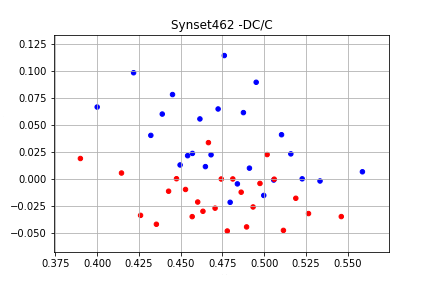
\includegraphics[width=0.45\textwidth]{images/462-DC-C.png}		
\ 		
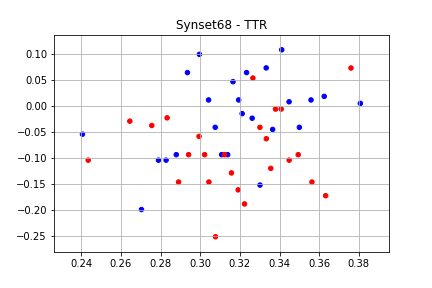
\includegraphics[width=0.45\textwidth]{images/68-TTR.png}		
\end{center}
\caption{Over- and under-use of Germanic words as a function of proficiency. Left: synset 462 vs.\ English syntactic proficiency measure DC/C; right: synset 68 vs.\ English Lexical proficiency measure TTR.}
\label{fig:results}	
\end{figure}






\bibliographystyle{plainnat}
\bibliography{all}

\end{document}

References
